\documentclass[12pt]{article}
\usepackage{fullpage}
\usepackage[utf8]{inputenc}
\usepackage{graphicx}
\usepackage[english]{babel}
\usepackage{float}
\usepackage{natbib}
\usepackage{authblk}
\usepackage{url}
\usepackage[section]{placeins}
\usepackage{wrapfig, framed}

\title{\textbf{Project 6 Report : Dimensionality reduction techniques}}
\author{Sajal Kumar}
\date{}

\begin{document}
\maketitle

\section*{Implementation details on parameters}

My implementation uses all 3 methods : Principal Component Analysis, Linear Discriminant Analysis and  Kernel Principal Component Analysis on their default setting except the following general parameters that could be changed:

\begin{itemize}
\item \texttt{random\_state} : Random seed (set to 1 by default).
\item \texttt{n\_jobs} : Number of parallel threads allowed (set to 4 by default).
\end{itemize}

I also allows changes to the \texttt{gamme} parameter in Kernel PCA, denoted by \texttt{gamma\_kernel\_pca} in the cod (set to 1/n\_features by default).

Apart from the above mentioned parameter some other dimensionality reduction technique specific parameters were changed but were not provided to the user:

\begin{itemize}
\item PCA
\begin{itemize}
\item \texttt{n\_components} was set to 'mle'.
\item \texttt{svd\_solver} was set to 'full'.
\end{itemize}
\item Kernel PCA
\begin{itemize}
\item \texttt{kernel} was set to `rbf'.
\end{itemize}
\end{itemize}

Additionally, I implemented a \texttt{var\_explained} $\in [0,1]$ parameter that is used to determine the number of transformed attributes (principal components). It was set to 0.9 by default.

The above represents the `standard' setting for all regression methods when no parameter is changed. 

Logistic regression was used for the classification task. I used it at its default setting except :

\begin{itemize}
\item \texttt{fit\_intercept} was set to False.
\item \texttt{solver} was set to `sag'.
\item \texttt{multi\_class} was set to `ovr'.
\end{itemize}

\subsection*{\texttt{var\_explained} for Kernel PCA}

Both PCA and LDA provide access to the member variable \texttt{explained\_variance\_ratio\_}, however, Kernel PCA doesn't as it is no longer in the same space as the input $X$. After some online search, I found that \texttt{numpy.var} could be used to compute the variance of each transformed attribute and then \texttt{explained\_variance\_ratio\_}. Hence, I wrote a tiny script to calculate the variance related to quantities so that I could evaluate the 3 methods with limited bias.

\section*{Performance evaluation}

I computed the runtime, prediction on training data, prediction on testing data and dimension usage on the original data as well as the three (PCA, LDA, Kernel PCA) transformed data to judge the quality of results before and after dimensionality reduction. Dimension usage $\in [0, 1]$ was added to note the percentage of dimensions used to achieve \texttt{var\_explained} threshold. Since Kernel PCA is in a different space, the dimension usage for it was found to be greater than 1 for both data-sets.

\subsection*{Performance on Iris Data-set}

\begin{table}[!hptb]
\centering
\begin{tabular}{|l|c|c|c|c|}
\hline
\textbf{Info} & \textbf{Og} & \textbf{PCA} & \textbf{LDA} & \textbf{KernelPCA} \\\hline
\textbf{runtime} & NA &	 0.001 & 0.002 & 1.83 \\
\textbf{pred on train} & 0.87 & 0.84 & 0.66 & 0.99 \\
\textbf{pred on test} & 0.8 & 0.73 & 0.66 & 0.86 \\
\textbf{dim usage} & 1 & 0.5 & 0.25 & 2.25 \\\hline
\end{tabular}
\caption{Result on `Iris' data-set with `standard' configuration of original and transformed inputs.}
\end{table}

Table~1 shows the runtime (in seconds), prediction on training data, prediction on testing data and dimension usage for `Iris' data-set using the `standard' configuration on the original (Og) and transformed dataset. The data-set was scaled using the `StandardScaler' method from sklearn. The data was split into 70\% training and 30\% testing using stratified partition.  LDA performs the worst and Kernel PCA does the best, however, if we look at the dimension usage, it can be seen that Kernel PCA uses way a lot more dimensions, which may explain the improved performance.

\begin{figure}
\begin{minipage}{\linewidth}
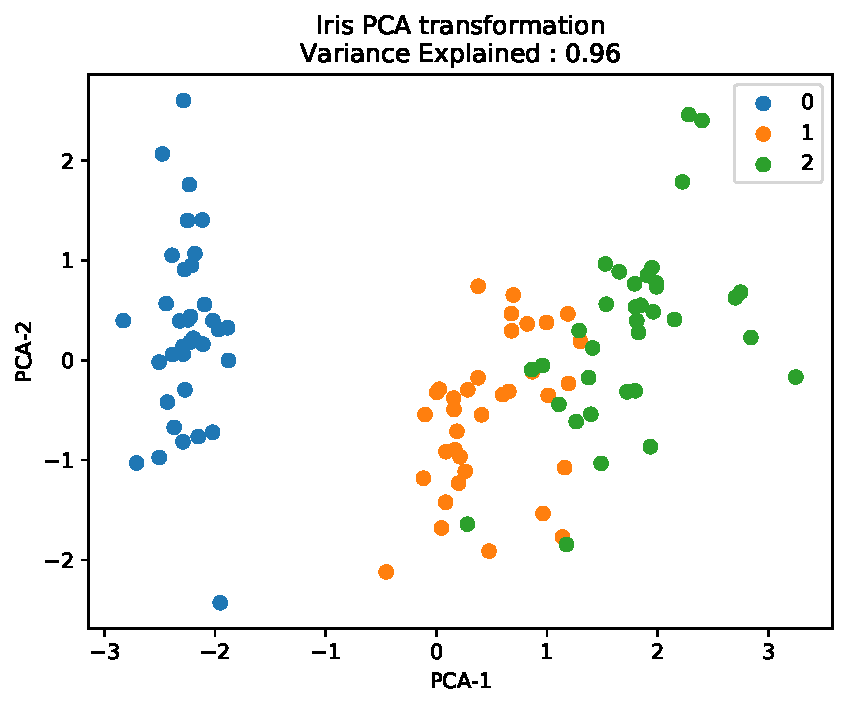
\includegraphics[width=0.32\linewidth]{Iris_PCA_top_two_components_.pdf}
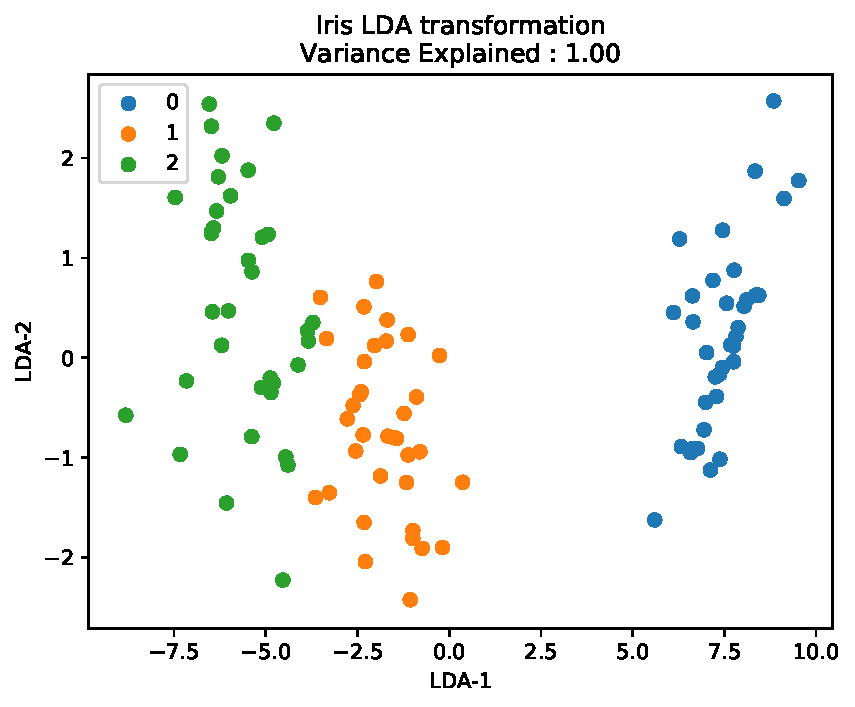
\includegraphics[width=0.32\linewidth]{Iris_LDA_top_two_components_.pdf}
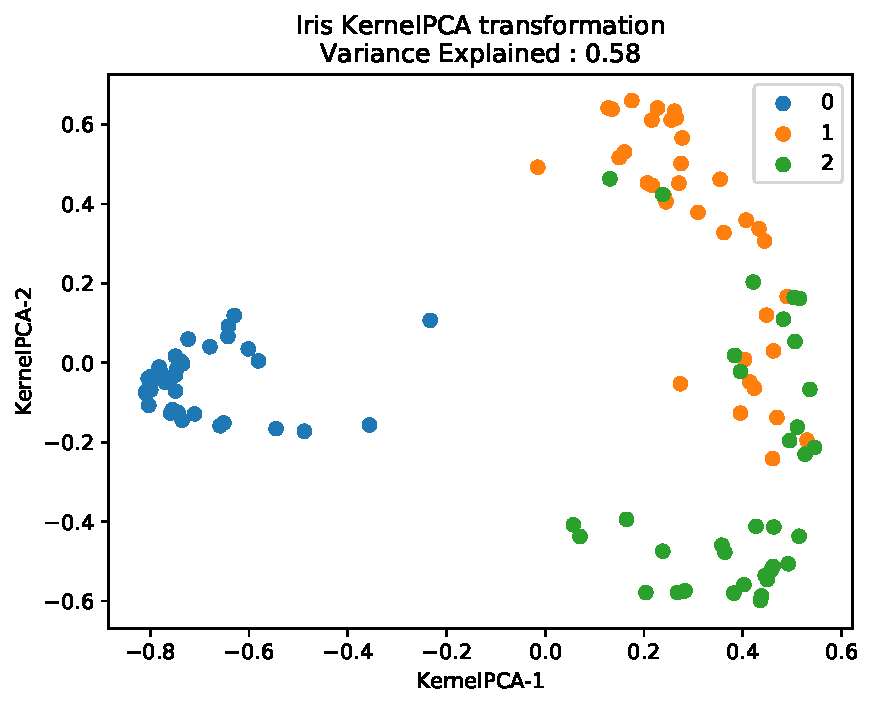
\includegraphics[width=0.32\linewidth]{Iris_KernelPCA_top_two_components_.pdf}
\end{minipage}
\caption{Top two principal components for each method.}
\end{figure}

Figure~1 shows the top two principal components for each method. It can be seen that while PCA and LDA do a good job capturing more than 95\% ($\geq 0.95$) variance, Kernel PCA can only capture 60\% variance. This clearly means that if one were to fix the number of principal components to two, Kernel PCA would show the worst performance.

\subsection*{Performance on Digits Data-set}

\begin{table}[!hptb]
\centering
\begin{tabular}{|l|c|c|c|c|}
\hline
\textbf{Info} & \textbf{Og} & \textbf{PCA} & \textbf{LDA} & \textbf{KernelPCA} \\\hline
\textbf{runtime} & NA & 0.14 & 0.025 & 2.78\\
\textbf{pred on train} & 0.93 & 0.90 &  0.78 & 0.97 \\
\textbf{pred on test} & 0.91 & 0.90 & 0.76 & 0.96 \\
\textbf{dim usage} & 1 & 0.48 & 0.09 & 5 \\\hline
\end{tabular}
\caption{Result on `Digits' data-set with `standard' configuration of original and transformed inputs.}
\end{table}

Table~2 shows the runtime (in seconds), prediction on training data, prediction on testing data and dimension usage for `Digits' data-set using the `standard' configuration on the original (Og) and transformed dataset. The data-set was scaled using the `StandardScaler' method from sklearn. The data was split into 70\% training and 30\% testing using stratified partition. Again LDA performs the worst and Kernel PCA does the best. This time around perhaps some explanation can be offered about LDA's poor performance, if we look at the dimension usage, LDA uses less than 1\% of the dimension, (even PCA uses almost 50\% of the dimensions) to achieve the target variance. Having less number of dimensions is probably what is hurting LDA as it is benefiting Kernel PCA that causes 5 times increase in dimension.

\begin{figure}
\begin{minipage}{\linewidth}
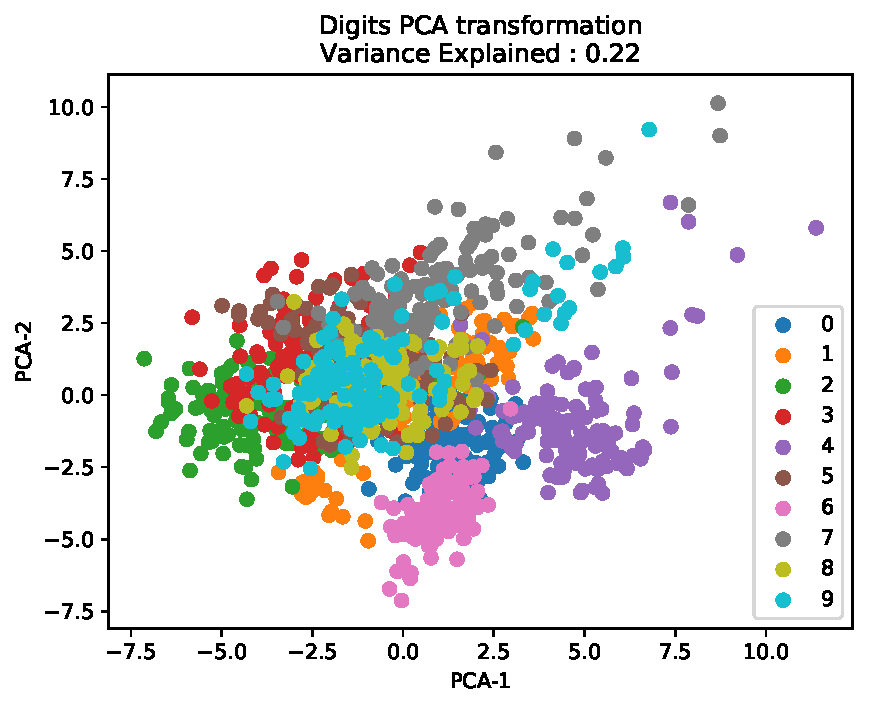
\includegraphics[width=0.32\linewidth]{Digits_PCA_top_two_components_.pdf}
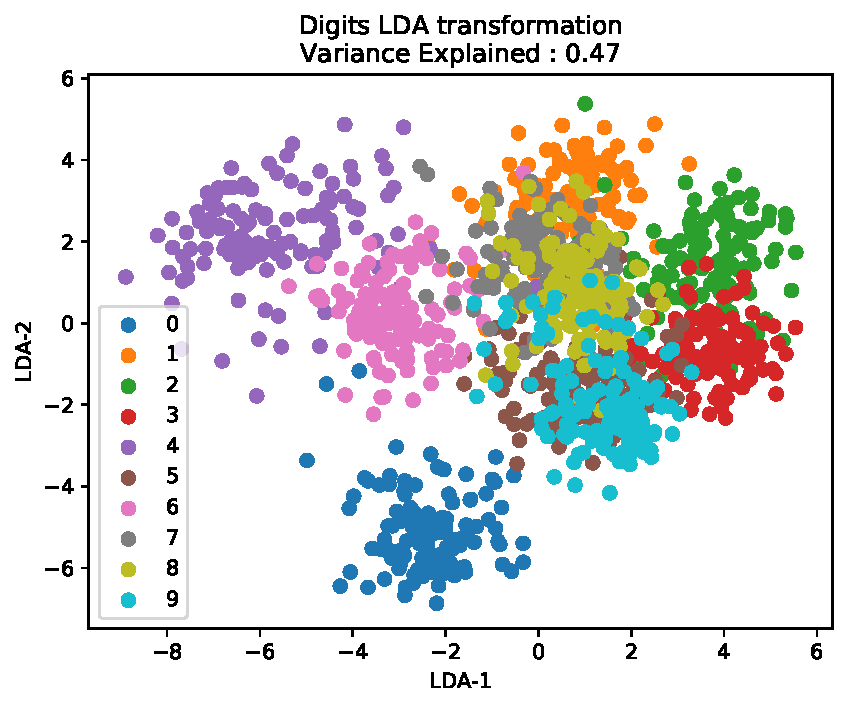
\includegraphics[width=0.32\linewidth]{Digits_LDA_top_two_components_.pdf}
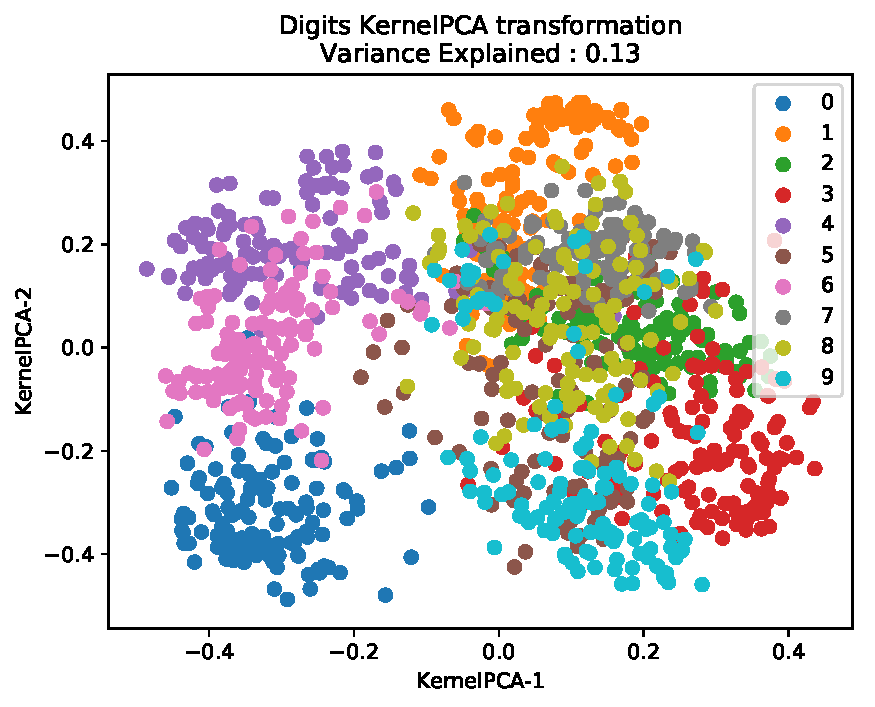
\includegraphics[width=0.32\linewidth]{Digits_KernelPCA_top_two_components_.pdf}
\end{minipage}
\caption{Top two principal components for each method.}
\end{figure}

Figure~2 shows the top two principal components for each method. No method could capture more than 90\% variance in the data set, however, LDA already captured about 50\% of the variance using just two components. Similar to that in the case of `Iris', Kernel PCA reports the least variance explanation score with two components in the `Digits' dataset.  Again this clearly means that fixing the number of principal components would degrade Kernel PCA's performance.

\section*{A more comprehensive evaluation}

Since most of the parameters were automatically computed, the only parameter I could have changed was \texttt{var\_explained}, while, there were no major change in the results when \texttt{var\_explained} was set to 0.98 for `Iris' data-set. LDA saw a major improvement in performance on the `Digits' data-set.

\begin{table}[!hptb]
\centering
\begin{tabular}{|l|c|c|c|}
\hline
\textbf{Info} & \textbf{Og} & \textbf{LDA-0.9} & \textbf{LDA-0.98} \\\hline
\textbf{runtime} & NA & 0.025 & 0.026\\
\textbf{pred on train} & 0.93 & 0.78 & 0.93 \\
\textbf{pred on test} & 0.91 & 0.76 & 0.91 \\
\textbf{dim usage} & 1 & 0.09 & 0.14 \\\hline
\end{tabular}
\caption{Improvement in LDA's performance for `Digits' data-set with \texttt{var\_explained} set to 0.98}
\end{table}

Table~3 shows the performance improvement for LDA, wherein, it is now using 14\% of the dimensions. Interestingly, for  \texttt{var\_explained}=0.98, the accuracy for LDA exceeded that of PCA by 1.5\% on both training and testing.

\end{document} 